\section{Premi\`eres approches}

\subsection{Notion de service Web}

\begin{frame}{Notion de service Web}
	\begin{block}{D\'efinition}
		\begin{itemize}
			\item Application accessible par le r\'eseau
			\item Ind\'ependant de tous langages
			\item Communication avec un client
			
		\end{itemize}
		
	\end{block}
	
	\begin{block}{Architecture}
		\begin{itemize}
			\item Architecture SOA : distributions de services
			\item \'Echanges : SOAP
			\item Description : WSDL
			\item D\'ecouverte : UDDI

		\end{itemize}
		
	\end{block}
	
\end{frame}

%%%%%%%%%%%%%%%%%%%%%%%%%%%%%%%%%

\begin{frame}{Notion de service Web}
	\begin{figure}[h]
		\centering
		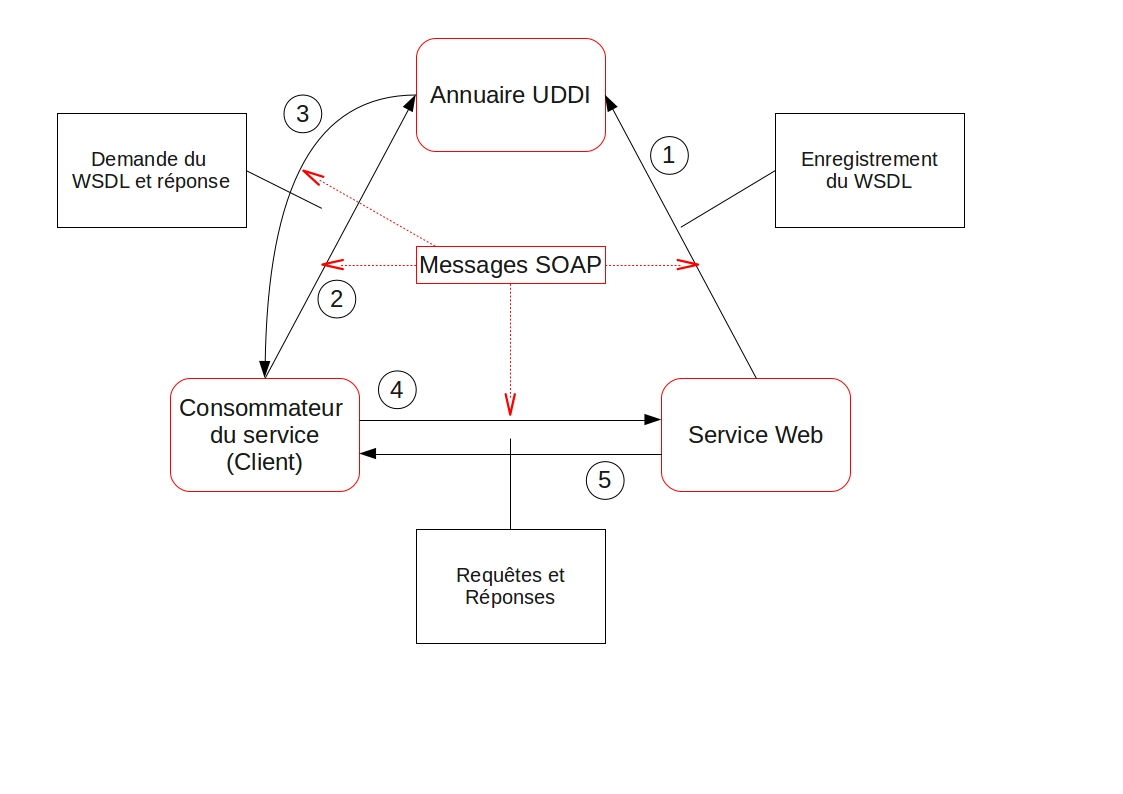
\includegraphics[scale=0.30]{schemaServiceWeb.jpg}
		
	\end{figure}
		
\end{frame}

%%%%%%%%%%%%%%%%%%%%%%%%%%%%%%%%%

\begin{frame}{Notion de service Web}
	\begin{block}{API JAX-WS}
		\begin{itemize}
			\item API Java pour les services Web
			\item Diff\'erentes m\'ethodes de d\'eveloppememt
			\item Facilit\'e avec NetBeans et GlassFish
		
		\end{itemize}

	\end{block}

\end{frame}

%%%%%%%%%%%%%%%%%%%%%%%%%%%%%%%%%

\subsection{Architecture du projet}

\begin{frame}{Architecture du projet}
	\begin{figure}[h]
		\centering
		\only<1>{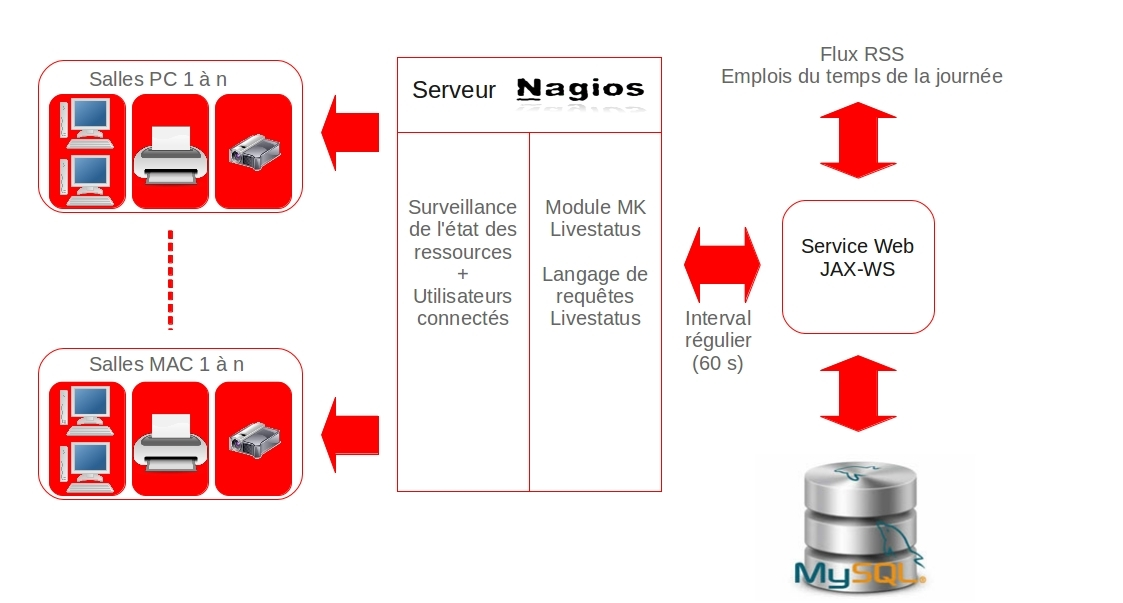
\includegraphics[scale=0.30]{architectureProjetServiceWeb.jpg}}
		\only<2>{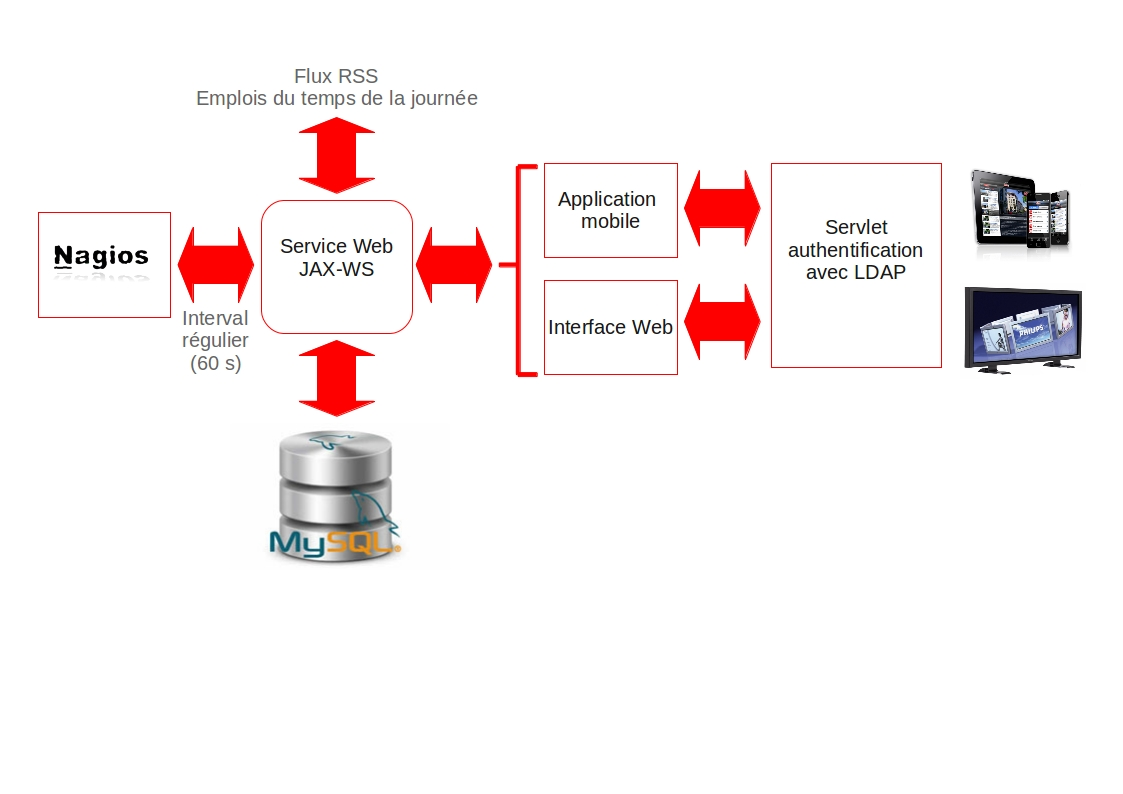
\includegraphics[scale=0.275]{architectureProjetAffichage.jpg}}
			
	\end{figure}
	
\end{frame}

%%%%%%%%%%%%%%%%%%%%%%%%%%%%%%%%%

\subsection{Outils utilis\'es}

\begin{frame}{Surveillance des ordinateurs}
	\begin{figure}[h]
		\centering
		
\includegraphics[scale=0.30]{nagiosLogo.jpg}
			
	\end{figure}
	
	\begin{block}{Nagios}
		\begin{itemize}
			\item Surveillance syst\`eme et r\'eseau
			\item Logiciel libre
			\item Interface graphique
		
		\end{itemize}

	\end{block}
	
\end{frame}

%%%%%%%%%%%%%%%%%%%%%%%%%%%%%%%%%

\begin{frame}{Surveillance des ordinateurs}
	\begin{block}{Module MKLivestatus}
		\begin{itemize}
			\item Int\'egr\'e au processus de Nagios
			\item Socket de communication
			\item \textit{Livestatus Query Language}
		
		\end{itemize}

	\end{block}
	
	\begin{block}{Quelques chiffres}
		\begin{itemize}
			\item Initialement
			\begin{itemize}
				\item Campus de New Cavendish
				\item 31 salles informatiques
				\item Environ 600 PC
			
			\end{itemize}
			
			\item Actuellement
			\begin{itemize}
				\item Presque toutes les salles
				\item 102 salles informatiques dont 3 pour les MAC
				\item 1920 PC et 63 MAC
			
			\end{itemize}
		
		\end{itemize}

	\end{block}
	
\end{frame}

%%%%%%%%%%%%%%%%%%%%%%%%%%%%%%%%%

\begin{frame}{Autres outils}
	\begin{figure}[h]
		\centering
		\subfloat{
\includegraphics[scale=0.242]{netbeansLogo.jpg}}
		\qquad
		\subfloat{
\includegraphics[scale=0.242]{glassfishLogo.jpg}}
		\qquad
		\subfloat{
\includegraphics[scale=0.3]{mysqlLogo.jpg}}

	\end{figure}

	\begin{block}{Autres outils}
		\begin{itemize}
			\item IDE NetBeans
			\item Serveur d'application GlassFish
			\item SGBD MySQL
		
		\end{itemize}

	\end{block}
	
\end{frame}

%%%%%%%%%%%%%%%%%%%%%%%%%%%%%%%%%

\begin{frame}{Choix du format de retour du service Webl}
	\begin{block}{Les recherches}
		\begin{itemize}
			\item Texte structur\'e
			\item Objet s\'erialisable
			\item XML
			\item JSON
		
		\end{itemize}

	\end{block}
	
	\begin{block}{Le choix}
		\begin{itemize}
			\item JSON
			\item Simple et rapide
			\item Langage d'\'echange id\'eal
		
		\end{itemize}

	\end{block}

\end{frame}



\subsection{Organisation du travail}

\begin{frame}{Organisation du travail}
	\begin{figure}[h]
		\centering
		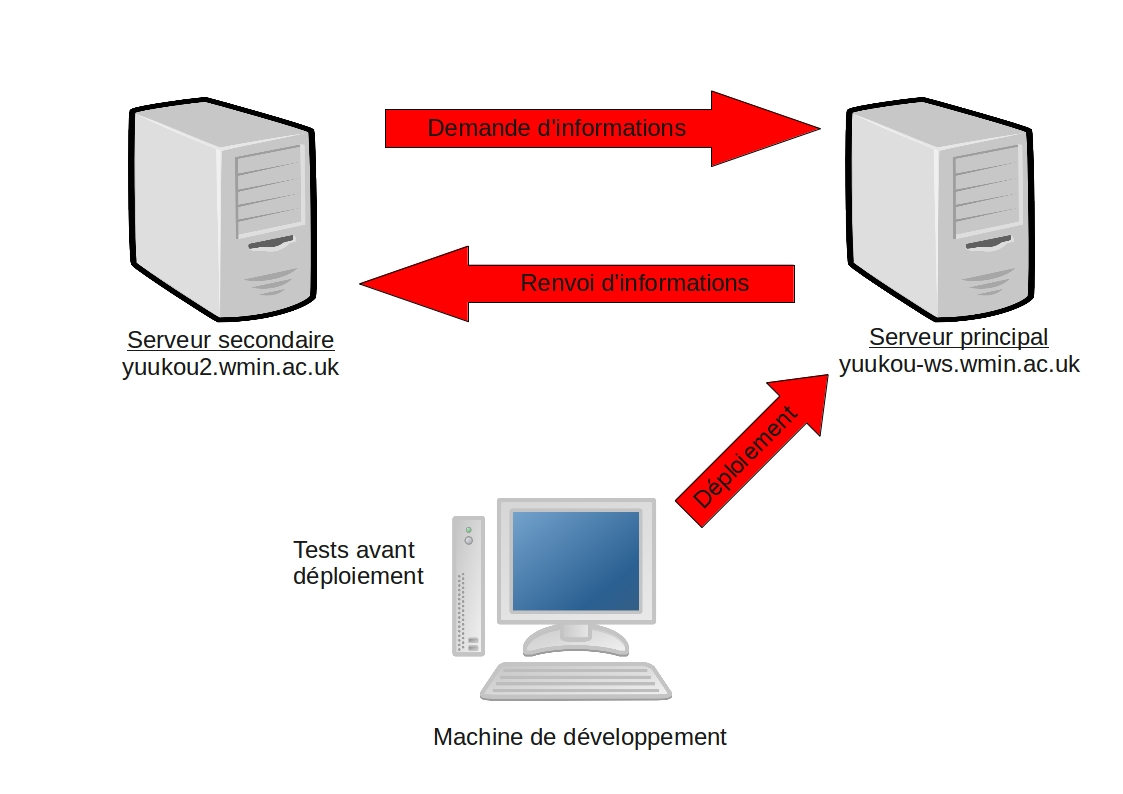
\includegraphics[scale=0.242]{gestionProjet.jpg}

	\end{figure}

\end{frame}














